\begin{figure}[!h]
	\centering
	\subbottom[original image\label{fig:egbfrseg}]{
		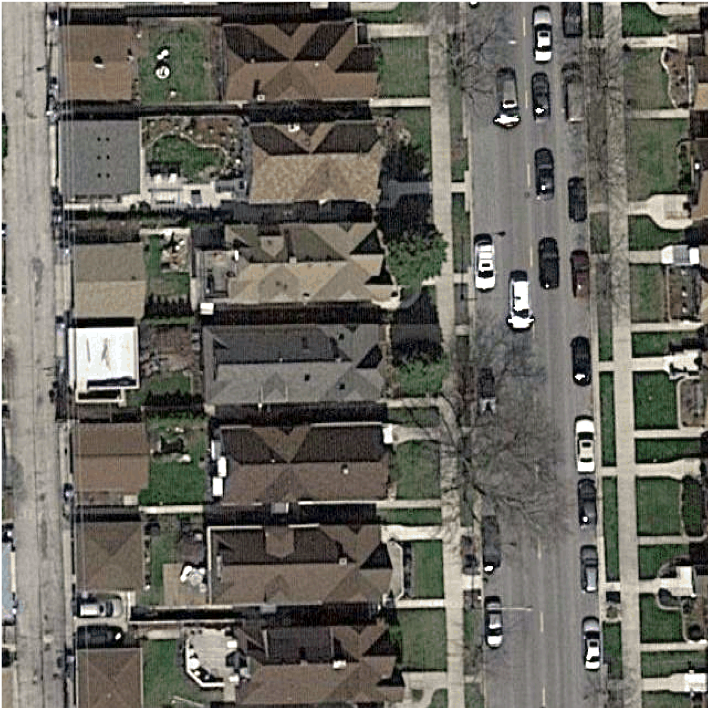
\includegraphics[width=\figfigfig\textwidth]{1-01-0.png}
	}
	\subbottom[segmentation result\label{fig:egaftseg}]{
		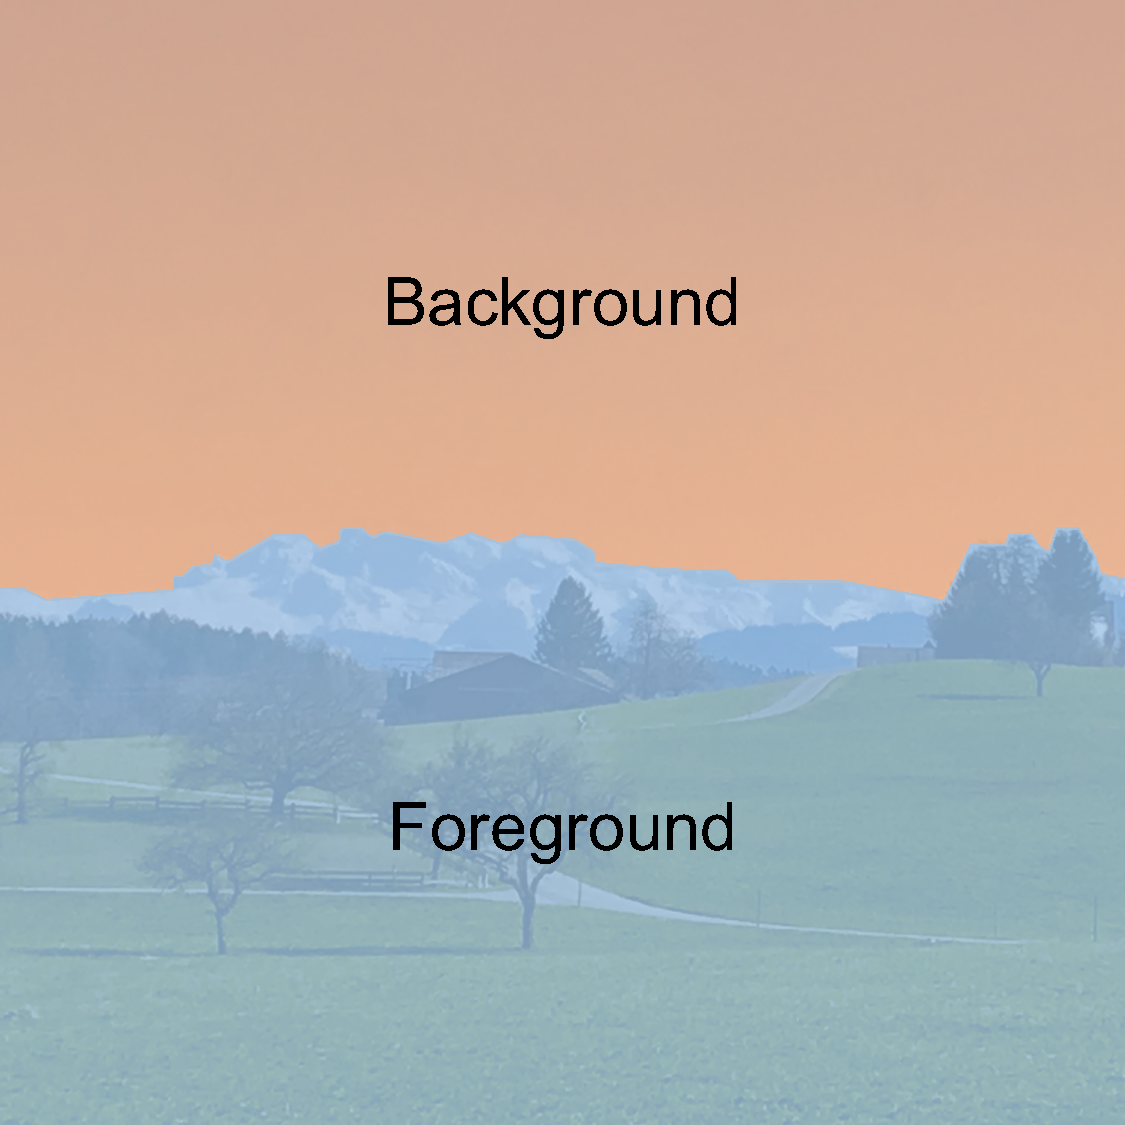
\includegraphics[width=\figfigfig\textwidth]{1-01-1.pdf}
	}
	\subbottom[alpha composition\label{fig:egmrgseg}]{
		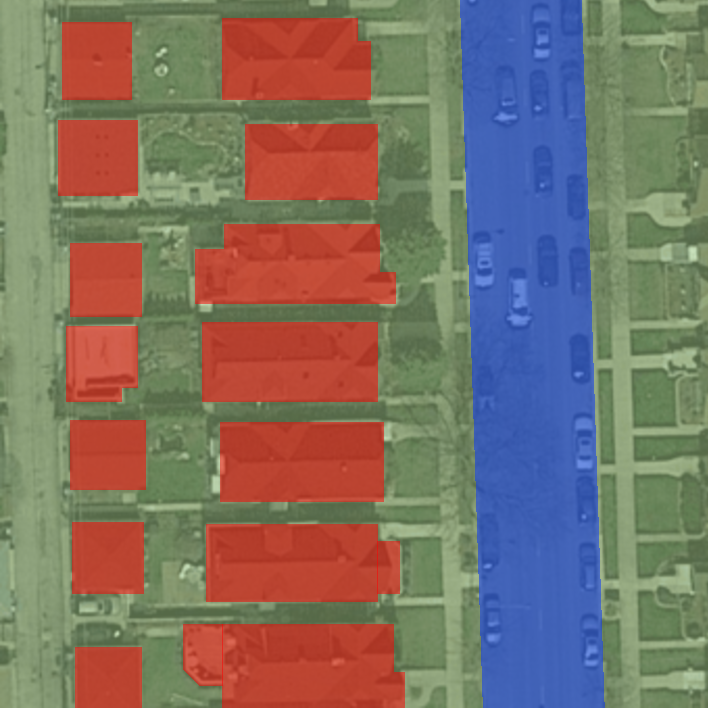
\includegraphics[width=\figfigfig\textwidth]{1-01-2.pdf}
	}
    \caption[Example of segmentation in aerial image.]{Example of segmentation in aerial image. The original image (a) is an area of Chicago. In (b), red color denotes buildings, blue color denotes roads, green color denotes background. (c) is (a) overlaid by (b) for clearness.}
	\label{fig:egarlimgseg}
\end{figure}